\documentclass[border=2mm]{standalone}
 
% Required packages and libraries
\usepackage{tikz}
\usetikzlibrary{positioning, arrows, decorations.pathreplacing}
% \usetikzlibrary{automata, positioning, arrows}
 

\begin{document}
 
 
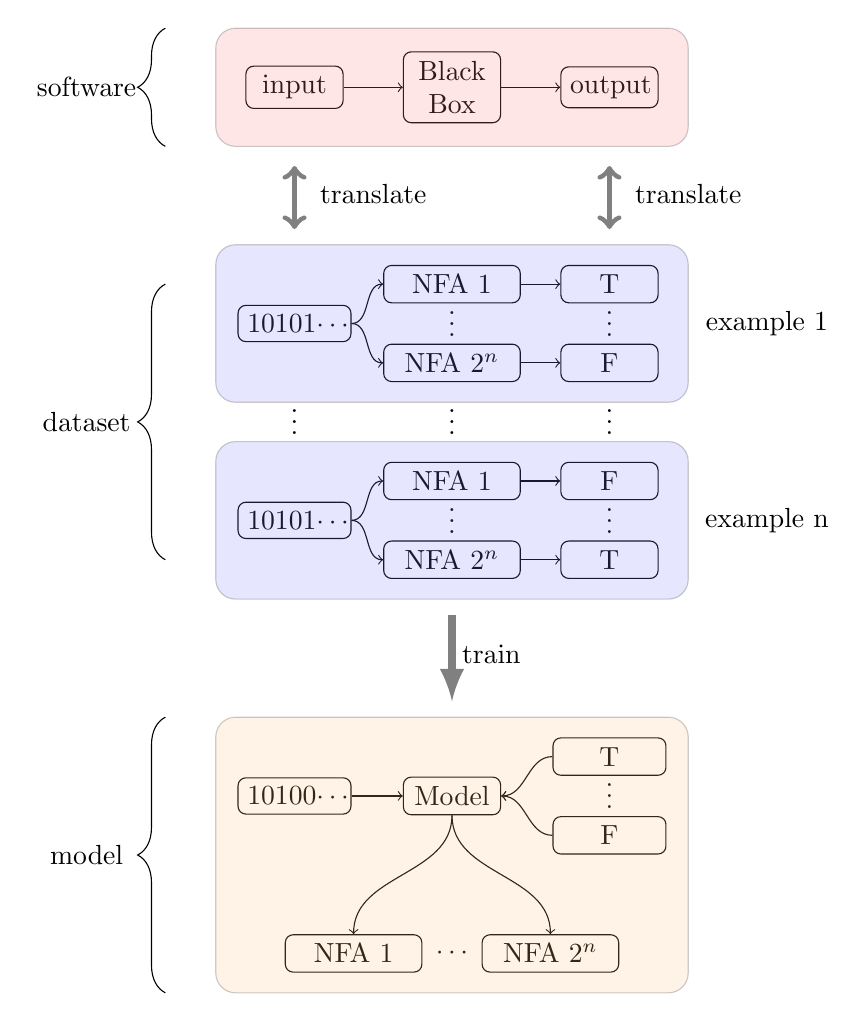
\begin{tikzpicture}[node distance = 2cm]

% --------- software --------- 
\node[draw, text width=10mm, rounded corners=1.0mm, align=center] at (0, 0) (BlackBox) {Black\\Box};
\node[draw, text width=10mm, rounded corners=1.0mm, align=center] at (-2, 0) (input) {input};
\node[draw, text width=10mm, rounded corners=1.0mm, align=center] at (2, 0) (output) {output};
\draw (input.east) edge[->, out=0,in=180] (BlackBox.west);
\draw (BlackBox.east) edge[->, out=0,in=180] (output.west);
\draw[rounded corners=2.5mm,fill=red!50, opacity=0.2] (-3, 0.75) -- (3, 0.75) -- (3, -0.75) -- (-3, -0.75) -- cycle;

% --------- dataset ---------
\node[draw, text width=12mm, rounded corners=1.0mm, align=center] at (-2, -3) (input) {10101$\cdots$};
\node[draw, text width=15mm, rounded corners=1.0mm, align=center] at (0, -2.5) (NFA1) {NFA $1$};
\node[rounded corners=1.0mm, align=center] at (0, -2.9) {$\vdots$};
\node[draw, text width=15mm, rounded corners=1.0mm, align=center] at (0, -3.5) (NFA2) {NFA $2^n$};
\node[draw, text width=10mm, rounded corners=1.0mm, align=center] at (2, -2.5) (output1) {T};
\node[rounded corners=1.0mm, align=center] at (2, -2.9) {$\vdots$};
\node[draw, text width=10mm, rounded corners=1.0mm, align=center] at (2, -3.5) (output2) {F};
\draw (input.east) edge[->, out=0,in=180] (NFA1.west);
\draw (input.east) edge[->, out=0,in=180] (NFA2.west);
\draw (NFA1.east) edge[->, out=0,in=180] (output1);
\draw (NFA2.east) edge[->, out=0,in=180] (output2);
\draw[rounded corners=2.5mm,fill=blue!50, opacity=0.2] (-3, -2) -- (3, -2) -- (3, -4.0) -- (-3, -4.0) -- cycle;

\node[rounded corners=1.0mm, align=center] at (-2, -4.15) {$\vdots$};
\node[rounded corners=1.0mm, align=center] at (0, -4.15) {$\vdots$};
\node[rounded corners=1.0mm, align=center] at (2, -4.15) {$\vdots$};

\node[draw, text width=12mm, rounded corners=1.0mm, align=center] at (-2, -5.5) (input) {10101$\cdots$};
\node[draw, text width=15mm, rounded corners=1.0mm, align=center] at (0, -5) (NFA1) {NFA $1$};
\node[rounded corners=1.0mm, align=center] at (0, -5.4) {$\vdots$};
\node[draw, text width=15mm, rounded corners=1.0mm, align=center] at (0, -6) (NFA2) {NFA $2^n$};
\node[draw, text width=10mm, rounded corners=1.0mm, align=center] at (2, -5) (output1) {F};
\node[rounded corners=1.0mm, align=center] at (2, -5.4) {$\vdots$};
\node[draw, text width=10mm, rounded corners=1.0mm, align=center] at (2, -6) (output2) {T};
\draw (input.east) edge[->, out=0,in=180] (NFA1.west);
\draw (input.east) edge[->, out=0,in=180] (NFA2.west);
\draw (NFA1.east) edge[->, out=0,in=180] (output1);
\draw (NFA2.east) edge[->, out=0,in=180] (output2);
\draw[rounded corners=2.5mm,fill=blue!50, opacity=0.2] (-3, -4.5) -- (3, -4.5) -- (3, -6.5) -- (-3, -6.5) -- cycle;

% --------- model ---------
\node[draw, text width=12mm, rounded corners=1.0mm, align=center] at (-2, -9) (input) {10100$\cdots$};
\node[draw, text width=10mm, rounded corners=1.0mm, align=center] at (0, -9) (Model) {Model};
\node[draw, text width=12mm, rounded corners=1.0mm, align=center] at (2, -8.5) (output1) {T};
\node[rounded corners=1.0mm, align=center] at (2, -8.9) (output2) {$\vdots$};
\node[draw, text width=12mm, rounded corners=1.0mm, align=center] at (2, -9.5) (output2) {F};
\node[draw, text width=15mm, rounded corners=1.0mm, align=center] at (-1.25, -11) (NFA1) {NFA $1$};
\node[rounded corners=1.0mm, align=center] at (0, -11) (NFAs) {$\cdots$};
\node[draw, text width=15mm, rounded corners=1.0mm, align=center] at (1.25, -11) (NFA2) {NFA $2^n$};
\draw (input.east) edge[->, out=0,in=180] (Model.west);
\draw (output1.west) edge[->, out=180,in=0] (Model.east);
\draw (output2.west) edge[->, out=180,in=0] (Model.east);
\draw (Model.south) edge[->, out=270,in=90] (NFA1.north);
\draw (Model.south) edge[->, out=270,in=90] (NFA2.north);
\draw[rounded corners=2.5mm,fill=orange!50, opacity=0.2] (-3, -8) -- (3, -8) -- (3, -11.5) -- (-3, -11.5) -- cycle;

\draw [<->, line width=2pt, black!50] (-2, -1) to (-2, -1.8);
\draw [<->, line width=2pt, black!50] (2, -1) to (2, -1.8);
\draw [-latex, line width=3pt, black!50] (0, -6.7) to (0, -7.8);

% --------------------------------
\node[rounded corners=1.0mm, align=center] at (-1, -1.35) {translate};
\node[rounded corners=1.0mm, align=center] at (3, -1.35) {translate};
\node[rounded corners=1.0mm, align=center] at (4, -3) {example 1};
\node[rounded corners=1.0mm, align=center] at (4, -5.5) {example n};
\node[rounded corners=1.0mm, align=center] at (0.5, -7.2) {train};
\draw [decorate,decoration={brace,amplitude=10pt},xshift=-4pt,yshift=0pt] (-3.5, -0.75) -- (-3.5, 0.75) node [black,midway,xshift=-10mm] {software};
\draw [decorate,decoration={brace,amplitude=10pt},xshift=-4pt,yshift=0pt] (-3.5, -6) -- (-3.5, -2.5) node [black,midway,xshift=-10mm] {dataset};
\draw [decorate,decoration={brace,amplitude=10pt},xshift=-4pt,yshift=0pt] (-3.5, -11.5) -- (-3.5, -8) node [black,midway,xshift=-10mm] {model};

% \node[draw, text width=1cm, align=center] at (-2, 0) (input) {input};
% \node[draw, text width=1cm, align=center] at (-2, 0) (input) {input};
% \node[draw, anchor=west] at (6, 1) (MatplotlibTimeSeriesVisualization) {MatplotlibTimeSeriesVisualization};
% \node[draw, anchor=west] at (6, 0) (QtTimeSeriesVisualization) {QtTimeSeriesVisualization};
% \node[draw, anchor=west] at (6, -1) (JSTimeSeriesVisualization) {JSTimeSeriesVisualization};
% \draw (TimeSeriesVisualization.east) edge[->, out=0,in=180] (MatplotlibTimeSeriesVisualization.west);
% \draw (TimeSeriesVisualization.east) edge[->, out=0,in=180] (QtTimeSeriesVisualization.west);
% \draw (TimeSeriesVisualization.east) edge[->, out=0,in=180] (JSTimeSeriesVisualization.west);

% \node[draw, anchor=west] at (0, -3.5) (TimeFreeVisualization) {TimeFreeVisualization};
% \node[draw, anchor=west] at (6, -2) (MatplotlibTimeFreeVisualization) {MatplotlibTimeFreeVisualization};
% \node[draw, anchor=west] at (6, -3) (QtTimeFreeVisualization) {QtTimeFreeVisualization};
% \node[draw, anchor=west] at (6, -4) (JSTimeFreeVisualization) {JSTimeFreeVisualization};
% \node[draw, anchor=west] at (6, -5) (MapTimeFreeVisualization) {MapTimeFreeVisualization};
% \draw (TimeFreeVisualization.east) edge[->, out=0,in=180] (MatplotlibTimeFreeVisualization.west);
% \draw (TimeFreeVisualization.east) edge[->, out=0,in=180] (QtTimeFreeVisualization.west);
% \draw (TimeFreeVisualization.east) edge[->, out=0,in=180] (JSTimeFreeVisualization.west);
% \draw (TimeFreeVisualization.east) edge[->, out=0,in=180] (MapTimeFreeVisualization.west);


% % --------- Data Preprocession --------- 
% \node[draw, anchor=west] at (0, 0-11) (Preprocessing) {Preprocessing};
% \node[draw, anchor=west] at (4, 3.5-11) (dataReduction) {.data\_reduction};
% \node[draw, anchor=west] at (4, 2.5-11) (noiseReduction) {.noise\_reduction};
% \node[draw, anchor=west] at (7, 1.5-11) (transformation) {.data\_transformation};
% \node[draw, anchor=west] at (7, 0.5-11) (integration) {.data\_integration};
% \node[draw, anchor=west] at (7, -0.5-11) (drop) {.drop\_missing\_data};
% \node[draw, anchor=west] at (7, -1.5-11) (fill) {.fill\_missing\_data};
% \node[draw, anchor=west] at (4, -2.5-11) (c2d) {.continues2discrete};
% \node[draw, anchor=west] at (4, -3.5-11) (d2c) {.discrete2continues};
% \draw (dataReduction.west) edge[->, densely dashed, out=180,in=10] (Preprocessing);
% \draw (noiseReduction.west) edge[->, densely dashed, out=180,in=10] (Preprocessing);
% \draw (transformation.west) edge[->, densely dashed, out=180,in=0] (Preprocessing.east);
% \draw (integration.west) edge[->, densely dashed, out=180,in=0] (Preprocessing.east);
% \draw (drop.west) edge[->, densely dashed, out=180,in=0] (Preprocessing.east);
% \draw (fill.west) edge[->, densely dashed, out=180,in=0] (Preprocessing.east);
% \draw (c2d.west) edge[->, densely dashed, out=180,in=-10] (Preprocessing);
% \draw (d2c.west) edge[->, densely dashed, out=180,in=-10] (Preprocessing);


% % --------- Data Mining --------- 
% \node[draw, anchor=east] at (-3, -4) (Classification) {Classification};
% \node[draw, anchor=east] at (-3, -6) (Regression) {Regression};
% \node[draw, anchor=east] at (-8, -4) (DecisionTree) {DecisionTree};
% \node[draw, anchor=east] at (-8, -5) (RandomForest) {RandomForest+CV};
% \node[draw, anchor=east] at (-8, -6) (NeuralNetwork) {NeuralNetwork};
% \draw (DecisionTree.east) edge[->, dotted, out=0,in=180] (Classification.west);
% % \draw (RandomForest.east) edge[->, dotted, out=0,in=180] (Classification.west);
% \draw (RandomForest.east) edge[->, dotted, out=0,in=180] (Regression.west);
% \draw (NeuralNetwork.east) edge[->, dotted, out=0,in=180] (Classification.west);
% \draw (NeuralNetwork.east) edge[->, dotted, out=0,in=180] (Regression.west);


% \node[draw, anchor=east] at (-3, -8) (AssociationMining) {AssociationMining};
% \node[draw, anchor=east] at (-8, -7.5) (candidate) {.gen\_candidate\_item\_set};
% \node[draw, anchor=east] at (-8, -8.5) (frequency) {.gen\_frequency\_item\_set};
% \draw (candidate.east) edge[->, densely dashed, out=0,in=180] (AssociationMining.west);
% \draw (frequency.east) edge[->, densely dashed, out=0,in=180] (AssociationMining.west);


% \node[draw, anchor=east] at (-3, -10) (SequentialPatternMining) {SequentialPatternMining};

% \draw (AssociationMining.south) edge[->, out=-90,in=90] (SequentialPatternMining.north);


% % --------- Boxes --------- 
% \draw[rounded corners=2.5mm,fill=blue!50, opacity=0.2] (-0.25, -5.5) -- (11.75, -5.5) -- (11.75, 1.5) -- (-0.25, 1.5) -- cycle;
% \draw[rounded corners=2.5mm,fill=orange!50, opacity=0.2] (-12, -10.5) -- (-2.75, -10.5) -- (-2.75, -3.5) -- (-12, -3.5) -- cycle;
% \draw[rounded corners=2.5mm,fill=red!50, opacity=0.2] (-0.25, -15) -- (10.75, -15) -- (10.75, -7) -- (-0.25, -7) -- cycle;


% \draw [-latex, line width=3pt, dotted, black!50] (2, -6.75) to (2, -5.75);
% \draw [-latex, line width=3pt, dotted, black!50] (-0.5, -8.75) to (-2.5, -8.75);
\end{tikzpicture}
 
 
\end{document}